\documentclass[aspectratio=169,10pt]{beamer}

\usepackage[utf8]{inputenc}
\usepackage{tikz}
\usepackage{forloop}

\usetheme{onion}

\title{Einführung in Tor}
\subtitle{KunterBuntesSeminar}

\date{\today}
\author{}
\institute{FBI}
\titlegraphic{\onionlogo{OnionBlack}}

\setlength{\parskip}{3mm}

%https://tex.stackexchange.com/questions/99316/symbol-for-external-links
\newcommand{\ExternalLink}{%
  \tikz[x=1.2ex, y=1.2ex, baseline=-0.05ex]{%
    \begin{scope}[x=1ex, y=1ex]
      \clip (-0.1,-0.1) 
      --++ (-0, 1.2) 
      --++ (0.6, 0) 
      --++ (0, -0.6) 
      --++ (0.6, 0) 
      --++ (0, -1);
      \path[draw, line width = 0.5, rounded corners=0.5] 
      (0,0) rectangle (1,1);
    \end{scope}
    \path[draw, line width = 0.5] (0.5, 0.5) -- (1, 1);
    \path[draw, line width = 0.5] (0.6, 1)   -- (1, 1) -- (1, 0.6);
  }
}



\begin{document}
  
  \maketitle
  
  \begin{frame}[fragile]{Outline}
    \begin{columns}
      \begin{column}{0.5\textwidth}
        \begin{itemize}
          \item Introduction to Tor
          \item Q\&A
          \item Tor Association for Hamburg
        \end{itemize}
      \end{column}
      \begin{column}{0.5\textwidth}
        \begin{center}
          \begin{overlayarea}{\textwidth}{0.5\textheight}
            \includegraphics[width=\textwidth]{img/Color.pdf}
          \end{overlayarea}
        \end{center}
      \end{column}
    \end{columns}
  \end{frame}
  
  
  \begin{frame}[fragile]{The Tor Project}
    \alert{Mission:} be the global resource for \textbf{technology}, \textbf{advocacy}, \textbf{research} and \textbf{education} in the ongoing pursuit of \textbf{freedom of speech}, \textbf{privacy rights online}, and \textbf{censorship circumvention}.
  \end{frame}
  
  
  \begin{frame}[fragile]{What is Tor?}
    \begin{itemize}
      \item Online anonymity
      \begin{itemize}
        \item FLOSS
        \item Open (volunteer-based) network
      \end{itemize}
      \item Community: researchers, developers, users, relay operators, [$\ldots$]
      \item U.S. 501(c)(3) non-profit organization
    \end{itemize}
  \end{frame}
  
  
  \begin{frame}[fragile]{What is Tor?}
    \begin{center}
      \href{https://metrics.torproject.org/userstats-relay-country.html}{\includegraphics[height=0.75\textheight]{img/userstats.pdf}}
      
      Estimated 2.000.000+ Tor users (daily)
    \end{center}
  \end{frame}
  
  
  \begin{frame}[fragile]{How does the Internet work?}
    \begin{columns}
      \begin{column}{0.5\textwidth}
        \begin{center}
          \href{https://commons.wikimedia.org/wiki/File:Internet_map_1024.jpg}{\includegraphics[height=0.75\textheight]{img/internet.jpg}}
        \end{center}
        \hbox{\thinspace{\small\itshape The Opte Project, \href{https://commons.wikimedia.org/wiki/File:Internet_map_1024.jpg}{Internet map 1024}, \href{https://creativecommons.org/licenses/by/2.5/legalcode}{CC BY 2.5}}}
      \end{column}
      \begin{column}{0.5\textwidth}
        \begin{itemize}
          \item A gigantic network of computers, servers and devices
          \item Every PC, server, device, refrigerator, $\ldots$ requires a unique identifier - \textbf{IP address}
          \item Internet is not the WWW (World Wide Web)
          \item Internet is the infrastructure
          \item Web is a service of this infrastructure
        \end{itemize}
      \end{column}
    \end{columns}
  \end{frame}
  
  
  \begin{frame}[fragile]{How does the Internet work?}
    On the Internet we are sending (a lot) of private data:
    \begin{itemize}
      \item Source/destination IP address
      \begin{itemize}
        \item Geographical location
      \end{itemize}
      \item WWW
      \begin{itemize}
        \item Web browser
        \item Operating system
        \item Addons and extensions
      \end{itemize}
      \item Other services: e-mail, telephone, chat (IRC, IM), file sharing, $\ldots$
    \end{itemize}
  \end{frame}
  
  
  \begin{frame}[fragile]{Understanding your threat model}
    \emph{I use encryption (HTTPS, ...) my ISP cannot see my traffic!}
    
    Maybe it cannot see your traffic (in cleartext), \textbf{but} it tracks:
    \begin{itemize}
      \item Websites visited
      \item Location logs
      \item IP address logs
      \item \ldots archived for x time: data retention
    \end{itemize}
  \end{frame}
  
  
  \begin{frame}[fragile]{VPN / Proxy providers}
    Often a single point of failure
    \begin{center}
      %draw.io
      \includegraphics<1>[width=0.8\textwidth]{img/vpn1.pdf}
      \includegraphics<2>[width=0.8\textwidth]{img/vpn2.pdf}
      \includegraphics<3>[width=0.8\textwidth]{img/vpn3.pdf}
    \end{center}
  \end{frame}
  
  
  \begin{frame}[fragile]{Anonymity: different interests for different user groups}
    \begin{center}
      %draw.io
      \includegraphics[width=0.8\textwidth]{img/interests.pdf}
    \end{center}
  \end{frame}
  
  
  % https://svn.torproject.org/svn/website/trunk/images/
  \begin{frame}[fragile]{How Tor works}
    \begin{center}
      \href{https://www.torproject.org/about/overview.html.en\#thesolution}{
        \includegraphics<1>[width=0.75\textwidth]{img/htw1.pdf}
        \includegraphics<2>[width=0.75\textwidth]{img/htw2.pdf}
        \includegraphics<3>[width=0.75\textwidth]{img/htw3.pdf}
      }
    \end{center}
    \only<1>{\hbox{\thinspace{\small\itshape \href{https://svn.torproject.org/svn/website/trunk/images/htw1.svg}{https://svn.torproject.org/svn/website/trunk/images/htw1.svg}}}}
    \only<2>{\hbox{\thinspace{\small\itshape \href{https://svn.torproject.org/svn/website/trunk/images/htw2.svg}{https://svn.torproject.org/svn/website/trunk/images/htw2.svg}}}}
    \only<3>{\hbox{\thinspace{\small\itshape \href{https://svn.torproject.org/svn/website/trunk/images/htw3.svg}{https://svn.torproject.org/svn/website/trunk/images/htw3.svg}}}}
  \end{frame}
  
  
  \begin{frame}[fragile]{Tor relay bandwidth}
    \begin{center}
      \only<1>{\href{https://metrics.torproject.org/bandwidth.html}{\includegraphics[width=0.9\textwidth]{img/bandwidth1.pdf}}}
      \only<2>{\href{https://metrics.torproject.org/bandwidth-flags.html}{\includegraphics[width=0.9\textwidth]{img/bandwidth2.pdf}}}
    \end{center}
  \end{frame}
  
  
  \begin{frame}[fragile]{Safety}
    Tor's safety comes from diversity
    \begin{itemize}
      \item Diversity of relays
      \item Diversity of users and reasons to use Tor
    \end{itemize}
    
    Transparency
    \begin{itemize}
      \item FLOSS
      \item Public design documents and specifications
      \item Public research
    \end{itemize}
  \end{frame}
  
  % 
  % \begin{frame}[fragile]{But what about the bad people?}
  % \begin{itemize}
  %  \item (remember) the millions of daily users
  %  \item Still a two-edged sword?
  %  \item Good people need Tor much more than bad people need it
  % \end{itemize}
  % \end{frame}
  
  
  \begin{frame}[fragile]{Onion services}
    Publish web sites and other services without needing to reveal the location of the site
    \begin{columns}
      \begin{column}{0.5\textwidth}
        \begin{itemize}
          \item Self authenticated
          \item End-to-end encrypted
          \item Built-in NAT punching
          \item Limit surface area
          \item No need to \emph{exit} from Tor
        \end{itemize}
      \end{column}
      \begin{column}{0.5\textwidth}
        \begin{center}
          \href{https://www.torproject.org/docs/onion-services.html.en}{\includegraphics[width=\textwidth]{img/onion5.png}}
        \end{center}
        \only<1>{\hbox{\thinspace{\small\itshape \href{https://www.torproject.org/images/tor-onion-services-5.png}{https://www.torproject.org/images/tor-onion-services-5.png}}}}
      \end{column}
    \end{columns}
  \end{frame}
  
  
  \begin{frame}[fragile]{Onion addresses}
    
    \begin{itemize}
      \item 3g2upl4pq6kufc4m.onion
      \item \alert{facebook}corewwwi.onion
      \item \alert{jamie}3vkiwibfiwucd6vxijskbhpjdyajmzeor4mc4i7yopvpo4p7cyd.onion
    \end{itemize}
  \end{frame}
  
  
  \begin{frame}[fragile]{Onion-service traffic}
    \begin{center}
      \href{https://metrics.torproject.org/hidserv-rend-relayed-cells.html}{\includegraphics[width=0.9\textwidth]{img/onionservice.pdf}}
    \end{center}
  \end{frame}
  
  
  \begin{frame}[fragile]{Onion services}
    \begin{columns}
      \begin{column}{0.5\textwidth}
        \begin{itemize}
          \item About 3\% of Tor's traffic has to do with onion services at all
          \item Onion services are evolving technology
          \item Terbium labs (and others) found ~7000 onion websites
          \item Also used for messengers and other applications
        \end{itemize}
      \end{column}
      \begin{column}{0.5\textwidth}
        \begin{center}
          \begin{overlayarea}{\textwidth}{0.5\textheight}
            \only<1>{\href{https://en.wikipedia.org/wiki/Facebookcorewwwi.onion}{\includegraphics[width=0.9\textwidth]{img/facebookonion.jpg}}}
            \only<2>{\href{https://securedrop.org/}{\includegraphics[width=0.9\textwidth]{img/securedrop.png}}}
            \only<3>{\href{https://ricochet.im/}{\includegraphics[width=0.9\textwidth]{img/ricochet.png}}}
            \only<4>{\href{https://onionshare.org/}{\includegraphics[width=0.9\textwidth]{img/onionshare.png}}}
          \end{overlayarea}
        \end{center}
      \end{column}
    \end{columns}
  \end{frame}
  
  
  \begin{frame}[fragile]{How can you help Tor?}
    \begin{itemize}
      \item Use \alert{Tor} and teach your friends
      \item Run a \alert{relay} or a \alert{bridge}
      \item Help fix -- and fix -- bugs
      \item Work on open research problems (\href{https://petsymposium.org/}{petsymposium.org})
      \item \href{https://donate.torproject.org/pdr}{Donate}
    \end{itemize}
  \end{frame}
  
  
  \begin{frame}[fragile]{Protect your privacy}
    \begin{center}
      \href{https://www.torproject.org/projects/torbrowser.html.en}{\includegraphics[height=0.85\textheight]{img/torbrowser.png}}
    \end{center}
  \end{frame}
  
  
  \begin{frame}[fragile]{Further information}
    \begin{itemize}
      \item \href{https://www.torproject.org/}{www.torproject.org}
      \item \href{https://support.torproject.org/}{support.torproject.org}
      \item \href{https://blog.torproject.org/}{Blog}
      \item \href{https://metrics.torproject.org/}{Metrics}
      \item \href{https://tails.boum.org/}{Tails}
    \end{itemize}
  \end{frame}
  

  \begin{frame}[fragile]{Artikel 10}
    2 people, running relays for years
    \begin{itemize}
      \item 1 exit since about 1 year
    \end{itemize}  
    \begin{center}
      \href{https://metrics.torproject.org/rs.html#search/family:F8BEB0F7AACC4F3EA6FF2C1FC19A9BD753887355}{\includegraphics[width=0.8\textwidth]{img/family.png}}
    \end{center}
    \textbf{We want to grow.}
  \end{frame}
  
  
  \begin{frame}[fragile]{Artikel 10}
    \begin{center}
      \href{https://metrics.torproject.org/rs.html#details/F8BEB0F7AACC4F3EA6FF2C1FC19A9BD753887355}{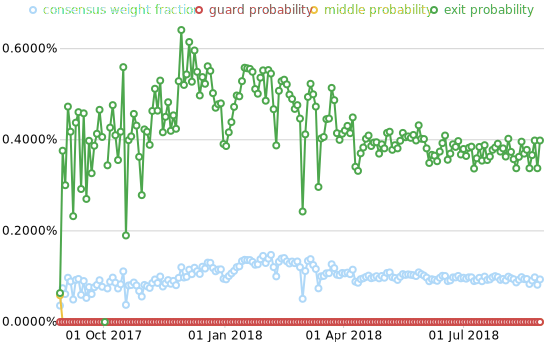
\includegraphics[height=0.8\textheight]{img/artikel10.pdf}}
    \end{center}
  \end{frame}
  
  
  \begin{frame}[fragile]{YATA -- Yet another Tor association?}
    \alert{Others:} Zwiebelfreunde, Digitalcourage, Artikel 5, Foundation for Applied Privacy  \href{https://torservers.net/partners.html}{\ExternalLink}
    
    \alert{Why?} Decentralize all the things!
    
    \alert{Artikel10!} Ein neuer Tor-Verein für Hamburg und Umgebung
  \end{frame}
  %TODO Bridges, hidden services vozriehen, tails
  
  \begin{frame}[fragile]{Stay in contact}
    \begin{center}
      \href{https://lists.riseup.net/www/info/artikel10}{\includegraphics[height=0.7\textheight]{img/mailinglist.png}}
      
      \href{https://lists.riseup.net/www/info/artikel10}{lists.riseup.net/www/info/artikel10}
    \end{center}
  \end{frame}


    %Q&A
  \maketitle

  
  \begin{frame}[fragile]{Sources}
    The presentation is based on \href{https://people.torproject.org/~andz/presentations/enucomp-keynote-parnaiba-br-2017.pdf}{https://people.torproject.org/~andz/presentations/enucomp-keynote-parnaiba-br-2017.pdf}.
  \end{frame}
  
\end{document}